%%%%%%%%%%%%%%%%%%%%%%%%%%%%%%%%%%%%%%%%%%%%%%%%%%%%%%%%%%%%%%%%%%%%%%%%%%%%%%%%
%2345678901234567890123456789012345678901234567890123456789012345678901234567890
%        1         2         3         4         5         6         7         8

\documentclass[letterpaper, 10 pt, conference]{ieeeconf}  % Comment this line out
                                                          % if you need a4paper
%\documentclass[a4paper, 10pt, conference]{ieeeconf}      % Use this line for a4
                                                          % paper

\IEEEoverridecommandlockouts                              % This command is only
                                                          % needed if you want to
                                                          % use the \thanks command
\overrideIEEEmargins
% See the \addtolength command later in the file to balance the column lengths
% on the last page of the document



% The following packages can be found on http:\\www.ctan.org
\usepackage{graphicx} % for pdf, bitmapped graphics files
%\usepackage{epsfig} % for postscript graphics files
%\usepackage{mathptmx} % assumes new font selection scheme installed
%\usepackage{times} % assumes new font selection scheme installed
%\usepackage{amsmath} % assumes amsmath package installed
%\usepackage{amssymb}  % assumes amsmath package installed

\title{\LARGE \bf
Flexible needle
}

\author{Guy Medan$^{1}$ and Leo Joskowicz$^{1}$% <-this % stops a space
\thanks{Grant}% <-this % stops a space
\thanks{$^{1}$HUJI
        {\tt\small josko at cs.huji.ac.il}}%
\thanks{Eyal, Ronen}%
}


\begin{document}



\maketitle
\thispagestyle{empty}
\pagestyle{empty}


%%%%%%%%%%%%%%%%%%%%%%%%%%%%%%%%%%%%%%%%%%%%%%%%%%%%%%%%%%%%%%%%%%%%%%%%%%%%%%%%
\begin{abstract}

Flexible needle abstract

\end{abstract}


%%%%%%%%%%%%%%%%%%%%%%%%%%%%%%%%%%%%%%%%%%%%%%%%%%%%%%%%%%%%%%%%%%%%%%%%%%%%%%%%
\section{INTRODUCTION}

Minimally invasive techniques are replacing open surgery for procedures such as biopsies.
In some procedures, a flexible needle is inserted under image guidance toward a target, either manually or using robotic actuators. 
In both cases visual feedback of the needle position within the tissue is required. 
Ultrasound imaging has been used to allow visual feedback, however it only offers a 2D cross section of the tissue.
CT guidance offers a 3D view of the needle insertion procedure at the expense of a large X-Ray dose to the patient since multiple scans are required as the needle is gradually inserted. Furthermore, image artifacts in CT are caused by the metallic needle during reconstruction, making it difficult to localize the tip of the needle with respect to the surrounding tissue. 
Dose reduction techniques focus on achieving a good quality of reconstruction using lower dose. However, in the common cases where a full baseline scan (without the needle) is available, reconstruction-free fractional scanning can be used. Fractional scanning refers to acquiring projection data from a sparse set of views, which is not large enough to allow reconstruction but enables registration with the baseline scan and localization of the needle in the repeat scan.
Visual feedback is particularly important for robotic driven needles, where the interaction of the needle and tissue is modeled in order to construct a control sequence realizing a planned insertion path. Such systems would benefit from mid-insertion feedback that would allow adjustments to the control sequence based on the achieved state of the needle insertion.

\section{PREVIOUS WORK}

\cite{wu2013automatic} \cite{engh2010percutaneous} describe implementations of a bevel-tip needle steering method using duty-cycle spinning of the needle, relying on its bending tendency due to asymmetry. Such systems model the needle-tissue interaction to execute a control sequence achieving a pre-planned trajectory. Imaging-based feedback is mentioned as a means to allow corrections of the control sequence mid-insertion by adjusting the planned trajectory based on the actual needle trajectory.
\cite{ben2018robotic} describe a robotic system for flexible needle insertion under CT guidance. A dual guiding mechanism is composed of a driver which advances the needle while a positioning unit steers it during insertion. A pre-planned trajectory is executed and amended during the insertion based on full repeated CT scans.
Earlier work \cite{glozman2007image} describes robotic flexible needle steering and a needle-tissue mechanical interaction model, where feedback is based on imaging of the needle.

Some works have proposed tracking needle trajectory in ultrasound imaging.

\cite{huo2015shape} reconstruct the bevel-tip flexible needle path from full CT slices by localizing points at which the needle intersects slice planes, and fitting a four-order polynomial to the collection of 3D points.

\cite{yaniv2010needle} use embedded electromagnetic fiducials for needle tracking under CT guidance, with operator input required to identify the needle tip in a full CT scan taken in-situ.

\section{MATERIALS AND METHOD}

We describe next an extension to flexible needles of our previous method \cite{medan2017reduced} for volume image-less rigid needle and patient tracking in interventional CT procedures based on fractional CT scanning. Similarly to our previous method, we begin by computing a sinogram-space rigid registration of the patient position in the CT scanner coordinate frame between a baseline scan without a needle, and a repeat scan with a needle introduced. The repeat scan is performed by sampling sparsely in the view angle domain (fractional scanning) and without reconstructing the CT image, while the baseline scan is assumed to be a full scan (sampled densely in the view angle domain). We use projection difference images, which are calculated by subtracting registered reprojected baseline scan images from the sparse set of repeat projection images. These highlight the differences between scans, which in our case is assumed to be the needle. The needle path is then traced in 3D space using only the projection difference images. The stages of our method are outlined below:
\begin{enumerate}
\item Rigid registration between the full baseline scan and sparse repeat scan, using our sinogram space rigid registration method \cite{medan2017sparse}.
\item Calculation of projection difference images using the registration obtained in the previous stage.
\item Spherical marker localization: we obtain a 3D localization of a spherical marker attached to the needle at a known distance from the tip, using the projection difference images.
\item Incrementally tracing the needle path: starting from the center of the marker obtained in the previous stage, we incrementally trace the needle path in 3D space using the projection difference images.
\item Display/feedback: the current location of the needle with respect to the baseline scan 3D image is displayed and/or used as feedback for further driving the needle toward the target.
\end{enumerate}
Steps 1-5 are repeated each time the needle is further inserted during the intervention, until the tip localization shows the desired target structure inside the patient is reached. Optionally, full CT scans for image reconstruction can be acquired during the procedure as needed. Our method uses the same sparse projection sampling pattern both for registration and for needle localization, avoiding additional scanning and image reconstruction so the radiation dose is a fraction of that required in image based methods. This allows frequent needle insertion and localization for feedback and accuracy without excessive radiation dose.

The rest of this section is organized as follows. 
% Section A provides a short background on the imaging characteristics of metallic objects in CT scanning. Section B describes the method materials, the composition and geometry of the spherical marker. Section C describes the projection space needle and marker localization method. Sections D and E elaborate on two key technical aspects of the method: needle and sphere localization in projection space and in 3D physical space.


\subsection{Marker localization}
Similarly to our previous method \cite{medan2017reduced}, the 3D center of the spherical marker is localized in three stages:

\begin{enumerate}

\item The 2D centers of the projected spherical marker are roughly localized in each of the $K$ projection difference images by correlating the difference projection image with a circular pattern.

\item The 2D projected marker centers are refined in each image by optimizing a cost function which takes into account the image gradients of the marker's surface.

\item The 3D position of the marker center $s$ is calculated by solving the inverse projection problem using the known projection geometry of the CT and the localized marker centers.

\end{enumerate}

\subsection{Incremental path reconstruction}

The path of the needle in 3D space is estimated by incrementally establishing a series of equidistant bezier curve control points along the path of the needle in 3D space $p_1, p_2, ..., p_i$, starting from the marker center $p_1=s$, which are used to construct a 3D curve $C_i$ tracing the path of the needle from the center of the spherical marker toward the tip, where $i$ is the number of control points in the incremental process. 

In each round a new point $p_{i+1}(\hat{n}) = p_i + \Gamma \hat{n}$ is established, where $\Gamma$ is the fixed distance between control points, and $\hat{n}$ is a direction to be determined via optimization. 
A 3D curve $C_{i+1}(\hat{n})$ is obtained from the control points $p_1, p_2, ..., p_i, p_{i+1}(\hat{n})$, and projected onto each of the $K$ view angles projection difference images to obtain projected curves $\bar{C}_{i+1}^j(\hat{n})$ where $j=1,...,K$ is the view angle index.
The direction $\hat{n}$ is obtained by optimizing a cost function designed to attain a minimum when the projection of the curve $C_{i+1}$ onto the set of projection difference images follows the needle path traced in the images:
\[ \textsf{C}_i(\theta_{\hat{n}}, \phi_{\hat{n}}) = -\sum_{j=1}^K{\int_{r \in \bar{C}_{i+1}^j(\hat{n})} {I_j(r)dl}} \]
where $ (\theta_{\hat{n}}, \phi_{\hat{n}}) $ is the representation of $ \hat{n} $ in spherical coordinates, and $r$ is the 2D coordinate along the projected path in projection difference image $I_j$. 
Accordingly, the orientation $\hat{n}_i$ of the $i$-th segment is obtained as $(\theta_{\hat{n}_i}, \phi_{\hat{n}_i}) = \textsf{argmin}_{\theta, \phi} \textsf{C}_i ( \theta, \phi)$.

The incremental process is stopped once the length of the 3D curve $C_{i+1}$ exceeds the known distance between the marker and needle tip. Then, the tip position is determined by trimming the last segment so that the overall length of the curve is equal to the known marker-tip distance.

\section{RESULTS}

To demonstrate our method we conducted an experiment consisting of flexible needles inserted into an abdomen phantom (CIRS model 57) and scanned using GE Discovery CT750HD scanner at GE Healthcare Haifa. The needles used were: a long 16 gauge (1.65mm outer diameter), and short 22 gauge (0.72mm outer diameter). For the long needle, the marker center was fixed at 235mm from the tip, and for the short needle at 135mm.
The reconstructed image size is $ 800 \times 800 \times 144 $ voxels, with spatial resolution of $0.58 \times 0.58 \times 1.25mm^3$. The detector array consists of 885 elements scanned at 984 views at regular intervals in the range [0⁰, 360⁰], where four slices were acquired in each full revolution. The data was re-binned from fan-beam to parallel rays’ representation of the projections.

At first a scan of the empty scanner bed was performed so that its sinogram can be subtracted from the following scans. Then, a full (dense sampling of view angles) baseline scan of the phantom was acquired, without the needle present. At each subsequent scan, the needle with attached spherical marker was inserted at a different location or different depth, and a full scan was acquired again. Sparse scanning was simulated by allowing the algorithm to access only a small subset of view angles.

The full baseline scan was registered to each sparse scan with needle inserted, using Radon-space rigid registration. The registration accuracy was evaluated as the root-mean-square of differences between voxel coordinates transformed by the calculated registration and by image-space registration of the reconstructed images. 
A sparse set of 24 evenly spaced view angles in the range $[0^\circ,180^\circ)$ was used for Radon-space registration and needle path reconstruction as previous experiments \cite{medan2017reduced} with a straight needle showed this selection offered a good trade-off between robustness and potential dose reduction.
The marker center and needle tip ground truth was obtained via manual localization on the reconstructed images.
Table \ref{results_table} summarizes the results of needle tip localization for the 7 scans in the dataset.

\section{Discussion}

\begin{table}[b]
\caption{Summary of experimental results}
\label{results_table}
\begin{center}
\begin{tabular}{|c||c|c|c|}
\hline
Scan ID & Reg. error [mm] & Marker error [mm] & Tip error [mm]\\
\hline
\hline
L1 & 1.4 & 1.9 & 2.6\\
\hline
L2 & 0.7 & 0.8 & 1.9\\
\hline
L3 & 0.6 & 0.3 & --\\
\hline
L4 & 1.0 & 0.8 & 2.0\\
\hline
S1 & 1.4 & 1.1 & 2.4\\
\hline
S2 & 1.2 & 4.5 & --\\
\hline
S3 & 1.5 & 0.9 & --\\
\hline
\end{tabular}
\end{center}
\end{table}

\begin{figure}[tpb]
\centering
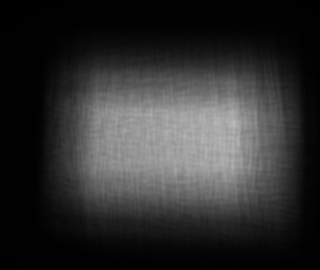
\includegraphics[width=6cm]{./example_raw.png}
\caption{Inductance of oscillation winding on amorphous
magnetic core versus DC bias magnetic field}
\label{figurelabel}
\end{figure}
   
\addtolength{\textheight}{-12cm}   % This command serves to balance the column lengths
                                  % on the last page of the document manually. It shortens
                                  % the textheight of the last page by a suitable amount.
                                  % This command does not take effect until the next page
                                  % so it should come on the page before the last. Make
                                  % sure that you do not shorten the textheight too much.

%%%%%%%%%%%%%%%%%%%%%%%%%%%%%%%%%%%%%%%%%%%%%%%%%%%%%%%%%%%%%%%%%%%%%%%%%%%%%%%%



%%%%%%%%%%%%%%%%%%%%%%%%%%%%%%%%%%%%%%%%%%%%%%%%%%%%%%%%%%%%%%%%%%%%%%%%%%%%%%%%



%%%%%%%%%%%%%%%%%%%%%%%%%%%%%%%%%%%%%%%%%%%%%%%%%%%%%%%%%%%%%%%%%%%%%%%%%%%%%%%%
\section*{APPENDIX}

Appendixes should appear before the acknowledgment.

\section*{ACKNOWLEDGMENT}

%%%%%%%%%%%%%%%%%%%%%%%%%%%%%%%%%%%%%%%%%%%%%%%%%%%%%%%%%%%%%%%%%%%%%%%%%%%%%%%%

\bibliographystyle{ieeetr}
\bibliography{flexible_needle}

\end{document}
